\chapter{Asking Billionaire Women How They Got Rich!}

This lecture is built out of street encounters, but it is not merely a collage of successful people. It has a real internal progression. We begin with scale before explanation, then move through structure, reinvestment, allocation, ownership, and finally a concentrated founder case in Sarah Blakely. Since no validated mathematical screenshots survive for this lecture, every equation and diagram in what follows is a cautious transcript-backed reconstruction. The aim is not to over-formalize the interviews, but to make their commercial logic legible without erasing their order, force, or local texture.

\section{Scale First, Explanation Later}

The lecture opens with a deliberate shock. A casual curbside question about becoming a millionaire is answered by a claim to billionaire status, followed by a self-reported peak year of extraordinary size. We are not yet told what to do with this number. That is the point. The lecture wants the magnitude on the page before it gives us doctrine.

\begin{equation}
Y_{\max} \approx \$1.2 \times 10^{9}.
\end{equation}

Here \(Y_{\max}\) is only a self-reported largest annual income, not an audited quantity. But the lecture uses it as a scale-setting device. Immediately after the shock comes the first serious economic question: where do the wealthiest people put their money? The answer is withheld for the moment. We are instead given the route of the episode: Beverly Hills first, Atlanta second, and Sarah Blakely as the promised culmination.

This is an important structural move. The lecture is not trying to derive a theorem from first principles. It is assembling a field of cases, and the early rhetorical violence of the opening is what gives later arithmetic its weight.

\section{Beverly Hills: Partial Access and Selective Doctrine}

The first Beverly Hills encounter is revealing precisely because it fails. A producer hints at very large revenue and then exits almost immediately. The transcript in this moment is too unstable to formalize cleanly, and we should resist the temptation to turn it into a hard quantitative case. What matters is the function of the beat: wealth is nearby, but access to the actual mechanism is incomplete.

The next interview is much denser. A finance-and-real-estate operator compresses several practical rules into a short span. We are told to invest in things we understand. When pressed for the best vehicle, she answers real estate; when pressed again, she narrows to residential. Time enters as well: she places her buying activity back in the 1990s, and geography enters with a distinction between coastal property and the tax advantages of red states.

\paragraph{Anecdote.} The lecture moves from a missed producer to a successful interview with a woman from finance who owns businesses and real estate.

\paragraph{Claim.} Rich operators prefer intelligible assets. In this case the preferred intelligible asset is residential real estate.

\paragraph{Mechanism.} The point is not merely that real estate went up. The point is that the owner could understand the asset class, hold it over time, and pair it with legal structure.

The same interview also contains remarks about hiring and trust that are very much the speaker's own and should remain attributed to her, not universalized into doctrine. The mathematically durable part of the segment is elsewhere: asset choice, long holding periods, and legal separation.

\section{Real Estate, LLCs, and the Protective Shell}

The lecture now narrows from the broad claim ``invest in what you understand'' to a more technical claim about how wealth is carried. The same operator says that each property sits inside its own LLC, and that the total number of LLCs exceeds fifty. The speaker calls the LLC a veil of protection. The host immediately recognizes the larger lesson: wealthy people do not leave structure to chance.

We can write the organizational rule schematically as
\begin{equation}
P_i \mapsto L_i,
\end{equation}
where \(P_i\) is the \(i\)-th property or business asset and \(L_i\) is the LLC shell that carries it. The count in the interview is
\begin{equation}
N_{\mathrm{LLC}} > 50.
\end{equation}

\subsection{Question \& Answer}

\paragraph{Question.} Why would we put each property into its own LLC instead of holding everything directly?

\paragraph{Answer.} The lecture's answer is not stated in legal jargon, but its logic is clear enough. If each asset sits inside its own shell, exposure is localized. The owner is not treating the portfolio as one undifferentiated block. She is separating it into compartments. The lecture does not derive this as a legal theorem, but the economic intuition is sharp: structure is part of wealth, not paperwork after wealth.

\begin{figure}[h]
\centering
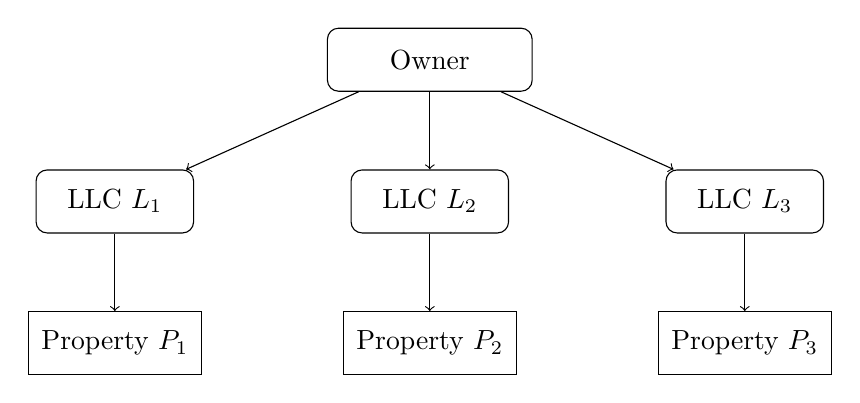
\begin{tikzpicture}[x=1cm,y=1cm]
\node[draw, rounded corners, minimum width=2.6cm, minimum height=0.8cm] (owner) at (0,4) {Owner};
\node[draw, rounded corners, minimum width=2.0cm, minimum height=0.8cm] (llc1) at (-4,2.2) {LLC \(L_1\)};
\node[draw, rounded corners, minimum width=2.0cm, minimum height=0.8cm] (llc2) at (0,2.2) {LLC \(L_2\)};
\node[draw, rounded corners, minimum width=2.0cm, minimum height=0.8cm] (llc3) at (4,2.2) {LLC \(L_3\)};
\node[draw, minimum width=2.2cm, minimum height=0.8cm] (p1) at (-4,0.4) {Property \(P_1\)};
\node[draw, minimum width=2.2cm, minimum height=0.8cm] (p2) at (0,0.4) {Property \(P_2\)};
\node[draw, minimum width=2.2cm, minimum height=0.8cm] (p3) at (4,0.4) {Property \(P_3\)};
\draw[->] (owner) -- (llc1);
\draw[->] (owner) -- (llc2);
\draw[->] (owner) -- (llc3);
\draw[->] (llc1) -- (p1);
\draw[->] (llc2) -- (p2);
\draw[->] (llc3) -- (p3);
\end{tikzpicture}
\caption{Transcript-backed reconstruction of the lecture's liability-shell logic: one entity per asset rather than one pooled structure.}
\end{figure}

At this point the lecture pauses for a sponsorship detour. It is worth preserving the pause, because it shows how quickly the host converts one operating practice into a general entrepreneurial slogan. Still, the durable content remains the structural point: the rich do not merely own; they own through forms.

\section{Ownership Without Dilution: The Beauty Founder Machine}

The next major case is the first one that behaves like a full business machine rather than a street fragment. A Beverly Hills beauty founder says she began in 1997, came from Romania under a communist regime, arrived with no money, no language, and no network, and later sold a company that she still describes as entirely hers before sale:
\begin{equation}
t_0 = 1997,\qquad t_s = 2018,\qquad s_f = 1,\qquad V_{\mathrm{beauty}} \approx \$3 \times 10^{9}.
\end{equation}

Again, the valuation language in the transcript is slightly rough, so \(V_{\mathrm{beauty}}\) should be treated as approximate. But the structural claim \(s_f=1\) matters greatly. No investors came in. Control stayed concentrated.

The lecture then shifts from biography to operating arithmetic. Her financial advice is plain: watch cash flow, treat EBITDA as central, do not spend aggressively, and put money back into the business. The easiest way to make this legible is with a retained-capital update rule:
\begin{equation}
K_{t+1} = K_t + \Pi_t - D_t.
\end{equation}
Here \(K_t\) is business capital at time \(t\), \(\Pi_t\) is operating surplus in a broad sense, and \(D_t\) is personal draw. The interview makes the sign of the rule unmistakable. \(D_t\) was kept small. She even gives a symbolic consumption marker:
\begin{equation}
C_{\mathrm{car}} \approx \$200.
\end{equation}
That number does not matter for its own sake. It matters because it stands for the lecture's anti-lifestyle-inflation principle.

\paragraph{Anecdote.} A founder drives a battered car, keeps her personal consumption low, and places generated money back into the firm.

\paragraph{Claim.} Cash flow matters more than appearance, and retained capital is what allows scale.

\paragraph{Mechanism.} A firm that reinvests can finance production, widen distribution, and survive long enough to learn.

\subsection{Question \& Answer}

\paragraph{Question.} If we keep reinvesting, how does that actually become scale rather than mere repetition?

\paragraph{Answer.} The lecture answers this in a sequence rather than a formula. More cash flow makes more production possible. More production makes wider distribution possible. Wider distribution expands the business's reach. Then a new channel can change the whole geometry of the firm.

We can summarize the sequence as
\begin{equation}
\text{cash flow} \rightarrow \text{production} \rightarrow \text{distribution} \rightarrow \text{scale}.
\end{equation}

The lecture then adds a second layer. Around 2012, the founder's daughter suggests Instagram as a substitute for constant travel. The firm begins posting images, supplying products to artists and creators, and riding tutorials and platform visibility into wider demand. In schematic form,
\begin{equation}
\text{travel-heavy promotion} \rightarrow \text{platform visibility} \rightarrow \text{viral proof} \rightarrow \text{distribution acceleration}.
\end{equation}

\begin{figure}[h]
\centering
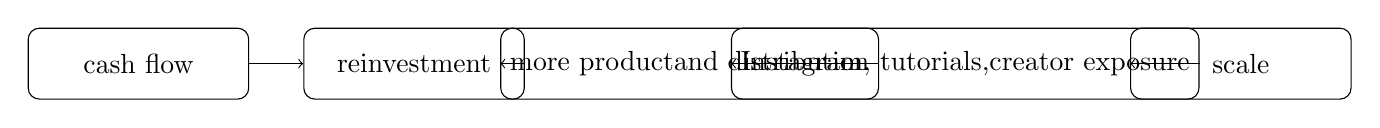
\begin{tikzpicture}[x=1cm,y=1cm]
\node[draw, rounded corners, minimum width=2.8cm, minimum height=0.9cm] (cf) at (-6,0) {cash flow};
\node[draw, rounded corners, minimum width=2.8cm, minimum height=0.9cm] (re) at (-2.5,0) {reinvestment};
\node[draw, rounded corners, minimum width=2.8cm, minimum height=0.9cm] (pd) at (1,0) {more product\\and distribution};
\node[draw, rounded corners, minimum width=2.8cm, minimum height=0.9cm] (ig) at (4.5,0) {Instagram, tutorials,\\creator exposure};
\node[draw, rounded corners, minimum width=2.8cm, minimum height=0.9cm] (sc) at (8,0) {scale};
\draw[->] (cf) -- (re);
\draw[->] (re) -- (pd);
\draw[->] (pd) -- (ig);
\draw[->] (ig) -- (sc);
\end{tikzpicture}
\caption{Transcript-backed reconstruction of the beauty founder's scaling path: reinvested cash flow first, then channel expansion, then social-media amplification.}
\end{figure}

The lecture does not stop with scale. It asks whether money buys happiness. The answer is more careful: money buys freedom, not fulfillment. This is an important late correction. The business machine is not denied, but it is placed inside a larger human frame.

\section{Atlanta: Portfolio Math and the Anti-Cash Rule}

After the Beverly Hills cases, the lecture resets itself through travel and expectation. Atlanta is not just another city. It is introduced as another field of wealth and as the route toward Sarah Blakely. The first strong Atlanta interview comes from a Wall Street-to-tech founder, and here the lecture finally gives its cleanest explicit arithmetic.

The speaker proposes a wealth partition:
\begin{align}
W &= W_{\mathrm{mkt}} + W_{\mathrm{cash}} + W_{\mathrm{alt}}, \\
W_{\mathrm{mkt}} &= 0.8W, \qquad
W_{\mathrm{cash}} = 0.1W, \qquad
W_{\mathrm{alt}} = 0.1W.
\end{align}
The transcript supplies the interpretation. Marketable securities mean stocks, bonds, mutual funds, and ETFs. Alternatives mean illiquid investments such as real estate and private investments. The time horizon attached to the alternative bucket is not instant liquidity but medium-term growth:
\begin{equation}
T_{\mathrm{alt}} \in [5,10]\ \text{years}.
\end{equation}

\subsection{Question \& Answer}

\paragraph{Question.} Where do the richest people actually put their money, and why not simply leave it in cash?

\paragraph{Answer.} The lecture's answer is that wealthy people give money a job description. Cash exists, but it is only one compartment and not the dominant one. Most wealth is placed where it can work.

A simple explicit example makes the lecture's rule concrete. If total wealth is
\[
W=\$100\,\text{million},
\]
then the interview's 80/10/10 split becomes
\[
W_{\mathrm{mkt}}=\$80\,\text{million},\qquad
W_{\mathrm{cash}}=\$10\,\text{million},\qquad
W_{\mathrm{alt}}=\$10\,\text{million}.
\]
The point is not that every rich person carries exactly this portfolio. The point is that the lecture insists on a difference between wealth held inertly and wealth assigned to productive compartments.

This is why the same interview makes the stronger claim that one does not save one's way to wealth. We can formalize the contrast minimally:
\begin{align}
W_{t+1}^{\mathrm{saved}} &= W_t + s_t, \\
W_{t+1}^{\mathrm{invested}} &= (1+r_t)W_t + s_t.
\end{align}
The distinction is elementary and it is exactly the one the lecture wants us to see. If the stock of wealth earns nothing, growth comes only from added contributions \(s_t\). If the stock is invested, then existing wealth participates in its own enlargement through \(r_t\).

\section{Belief, Ownership, and the Right to Be in the Room}

The same Atlanta interview refuses to remain merely arithmetical. After the portfolio split comes a psychological claim learned from Wall Street: the top \(1\%\) believe they belong in the room. They believe they deserve power. They believe they are supposed to be wealthy. The lecture is careful here. This is not a substitute for the arithmetic we have just seen. It is the disposition that allows a person to act on that arithmetic.

The speaker links that belief to biography: middle-class household, first in the family to attend college, first entrepreneur, first millionaire. She also links it to institutional exposure: she had seen wealthy people at close range and concluded that there was no metaphysical barrier separating them from everyone else. The lecture's phrasing becomes almost axiomatic at this point: wealth begins in the mind, but the key is ownership.

This is the right place to connect the softer language of belief with the harder language of control. Wage income matters, but the repeated doctrine of the lecture is that ownership alters the whole economic structure. Assets, companies, and retained claims have different dynamics from salary alone. The lecture does not give a formal theorem here, but by this point the theme is unmistakable: to believe that one belongs is not yet wealth, but it is often the precondition for taking the risks through which ownership becomes possible.

\section{Sarah Blakely and the Controlled Founder Path}

Sarah Blakely is the culminating case because her story concentrates nearly every theme that the lecture has been spreading across its earlier interviews. She begins with a finite sum of self-saved capital and refuses dilution from the start:
\begin{equation}
K_0 = \$5{,}000,\qquad T_{\mathrm{fax}} = 7\ \text{years},\qquad T_{\mathrm{self}} = 21\ \text{years},\qquad V_{\mathrm{sale}} = \$1.2 \times 10^{9}.
\end{equation}
The lecture's internal contrast is very sharp. Instead of fundraising, she chooses self-funding. Instead of splitting authority, she preserves it.

\subsection{Question \& Answer}

\paragraph{Question.} Should a founder give away ownership early in order to grow faster?

\paragraph{Answer.} Sarah Blakely's answer is cautious but firm. Whatever fraction one gives away, one must be willing to surrender the control attached to it. In minimal notation,
\begin{equation}
s_f' = 1-\alpha,
\end{equation}
where \(\alpha\) is the fraction sold and \(s_f'\) is the founder's retained economic claim. The interview's deeper point is qualitative rather than cap-table technical. Control matters because a founder may need to act on intuition before the numbers fully justify themselves. Her phrase is that intuition is not on a spreadsheet.

This gives the lecture a new pair of terms: data and intuition. It does not reject data. It claims that, in some founder settings, intuition reaches ahead of what current spreadsheets can certify.

The lecture then turns to rejection, and here again it prefers an operational rule to a sentimental one. Years of selling fax machines door to door trained her to treat rejection not as evidence of impossibility, but as part of the approach path to a yes. That is not a mathematical identity, but it is an update rule for conduct.

The lecture's next move is wonderfully concrete. Once she lands Neiman Marcus, she does not passively accept placement in an obscure corner of the hosiery department. She buys bins from Office Depot, places them at cash registers, and moves attention toward the product. This is a lesson in distribution politics: shelf position, traffic, and point of sale are not neutral. The founder acts where the customer actually is.

\subsection{Question \& Answer}

\paragraph{Question.} Should we talk about an idea immediately, or should we hold it privately until it is stronger?

\paragraph{Answer.} Sarah Blakely's answer is to wait. She says she kept the idea private for about a year:
\begin{equation}
\tau = 1\ \text{year}.
\end{equation}
The lecture's reasoning is subtle. Early ideas are fragile, and premature discussion recruits the ego too soon. Once ego enters, time is spent defending and explaining the idea rather than building it. In schematic form,
\begin{equation}
\text{ego involvement} \uparrow \;\Rightarrow\; \text{defense time} \uparrow.
\end{equation}
This is not a theorem. It is a founder heuristic. But it is a very good one, and it fits the lecture's repeated concern with preserving control over both ownership and attention.

The final conceptual turn in Sarah's interview is perhaps the strongest in the whole chapter. She did not enter a fashionable industry. She entered a declining one. Hosiery, as she describes it, was already in double-digit decline. Yet she noticed a live unsolved problem in women's clothing. Existing undergarments were too thick, too visible, too constricting. Her answer was not to chase the trend line but to redesign the object:
\begin{align}
\text{old undergarment} &=
\text{thick} + \text{visible} + \text{constricting}, \\
\text{new product} &=
\text{second-skin} + \text{lightweight} + \text{smooth silhouette}.
\end{align}
This is the lecture's most important product lesson. A declining category is not necessarily a dead category. It may simply be a category in which the underlying user problem has not yet been solved correctly.

What earlier appeared as scattered doctrine is now gathered together. Bet on oneself. Keep ownership where possible. Endure rejection. Intervene directly in distribution. Protect the idea while it is fragile. Solve a real problem, even in a tired market. By the time Sarah closes with ``solve a problem, bet on yourself, and have fun,'' the line no longer sounds motivational. It sounds earned.

\section{Summary}

The lecture begins with spectacle and ends with method. In between, it gives us a sequence of increasingly strong constructions. Wealth is allocated rather than hoarded. Assets are structured rather than pooled carelessly. Growth is financed through reinvestment rather than appearance. Ownership matters because control matters. Distribution matters because product alone is not enough. And even a declining industry can become the site of a decisive commercial breakthrough if the founder sees a problem that incumbents have learned not to see.

What makes the chapter work is that these points are not delivered as abstract laws from the outset. They emerge case by case. First we are shown scale. Then we are shown compartments, update rules, and choices. The lecture's commercial arithmetic is therefore modest in form but strong in consequence: separate the assets, keep capital at work, preserve control when it matters, and solve the concrete problem in front of the customer.